\documentclass[11pt]{article}
\usepackage{amsmath, amssymb}
\usepackage[margin=1in]{geometry}
\usepackage{xurl}
\usepackage[citestyle=authoryear,natbib=true,backend=biber,style=apa]{biblatex}
\usepackage{graphicx}
\usepackage{lineno}
\usepackage{setspace}
\usepackage{enumerate}
\usepackage{multirow}
\usepackage{multicol}
\usepackage{booktabs}
\usepackage{siunitx}
\sisetup{group-separator = {,},separate-uncertainty=true}

%% Set up bibliography
\bibliography{lit.bib}

%% For line numbers
\linenumbers

\begin{document}

\begin{titlepage}
    \begin{center}
        \vspace*{1cm}
        \large
        \textbf{Simplifying small area estimation with rFIA: a demonstration of tools and techniques}\\
         \normalsize
           \vspace{5mm}
         Hunter Stanke\textsuperscript{1,2}, Andrew O. Finley\textsuperscript{1}, and Grant M. Domke\textsuperscript{3}\\
         \vspace{5mm}
    
    \end{center}
    \small
    \textsuperscript{1}Department of Forestry, Michigan State University, East Lansing, MI, USA\\
    \textsuperscript{2}School of Environmental and Forest Sciences, University of Washington, Seattle, WA, USA\\
    \textsuperscript{3}Forest Service, Northern Research Station, US Department of Agriculture, St Paul, MN, USA\\ 
    \noindent \textbf{Corresponding Author}: Hunter Stanke, telephone: (269) 221-4745; email: stankehu@msu.edu

    \begin{abstract}
    \noindent The United States (US) Department of Agriculture Forest Service Forest Inventory and Analysis (FIA) program operates the national forest inventory of the US. Traditionally, the FIA program has relied on sample-based approaches---permanent plot networks and associated design-based estimators---to estimate forest variables across large geographic areas and long periods of time. These approaches generally offer unbiased inference on large domains but fail to provide reliable estimates for small domains due to low sample sizes. Rising demand for small domain estimates will thus require the FIA program to adopt non-traditional estimation approaches that are capable of delivering defensible estimates of forest variables at increased spatial and temporal resolution, without the expense of collecting additional field data. In light of this challenge, the development of small area estimation (SAE) methods---estimation techniques that support inference on small domains---for FIA data has become an active and highly productive area of research. Yet, SAE methods remain difficult to apply to FIA data, due in part to the complex data structures and inventory design used by the FIA program. Thus, we argue that a new suite of estimation tools (i.e., software) will be required to accommodate shifts in demand for inference on large geographic areas and long time periods to inference on small spatial and/or temporal domains. Herein, we present rFIA, an open-source R package designed to increase the accessibility of FIA data, as one such tool. Specifically, we present two case studies chosen to demonstrate rFIA's potential to simplify the application of a broad suite of SAE methods to FIA data: (1) estimation of contemporary county-level forest carbon stocks across the conterminous US using a spatial Fay-Herriot model; and (2) temporally-explicit estimation of multi-decadal trends in merchantable wood volume in Washington County, Maine using a Bayesian mixed-effects model. In both cases, we show that the application of SAE techniques offers considerable improvements in precision over FIA's traditional, post-stratified estimators. Finally, we offer a discussion of the potential role that rFIA and other open-source tools may play in accelerating the adoption of SAE techniques among users of FIA data.  
 

    \end{abstract}



\end{titlepage}



\section*{Introduction}


%% Introduce FIA, its research significance, and the need for small area estimators. Note that much work has been done on this front already, and this continues today. These methods may increase efficiency of estimators constructed from existing data, draw on auxiliary data sources to improve inference on small domains, or both.
The United States (US) Department of Agriculture Forest Inventory and Analysis (FIA) program conducts the US national forest inventory (NFI), collecting data describing the condition of forest ecosystems on a large network of permanent inventory plots distributed across all lands in the nation \citep{smith2002forest}. These data offer a unique and powerful resource for determining the extent, magnitude, and causes of long-term changes in forest health, timber resources, and forest landowner characteristics across large spatial domains in the US \citep{wurtzebach2020supporting}. The FIA program has traditionally relied on post-stratification to improve precision of point and change estimates \citep{westfall2011post, bechtold2005enhanced}, though like other NFIs \citep{breidenbach2012small, kohl2006sampling}, has experienced increased demand for estimates within smaller spatial, temporal, and biophysical extents than post-stratification can reasonably deliver (e.g., annual, stand-level estimates). The development of estimation techniques that support inference on small domains---referred to as small area estimation (SAE) methods---using FIA data is an active area of research, with considerable progress made in the last decade \citep{hou2021updating, coulston2021enhancing, schroeder2014improving, lister2020use}. SAE methods are numerous and diverse, though most seek to improve inference on small domains by making use of statistical models and auxiliary information that is correlated with the variable(s) of interest \citep{rao2015small}.

%% rFIA was originally designed to improve access to standard post-stratified estimators, aimed at alleviating some of the primary barriers to access. rFIA can also be particularly useful for 
Despite recent progress in the development of SAE methods, many users of FIA data are likely to find such techniques difficult to implement due to limitations in data accessibility and complexity in inventory design. Here, we demonstrate the potential of rFIA \citep{stanke2020rfia}, an open-source R package \citep{r2021}, to alleviate some of these hurdles. We developed rFIA to reduce barriers in data access that arise from complexity in data coding, database structure, and Structured Query Language used by the FIA program. Using a simple yet powerful design, rFIA implements the post-stratified, design-based estimation procedures described in \citet{bechtold2005enhanced} for over 60 forest variables and allows users to return intermediate summaries of all variables for use in modeling studies (i.e., plot, condition, and/or tree-level). Further, forest variables can be easily estimated for populations defined by any combination of spatial units (i.e., spatial polygons), temporal domains (e.g., most recent measurements), and/or biophysical attributes (e.g., species, site classifications). 

%% Some definitions and design principles guiding use of SAE methods in rFIA
The design-based, post-stratified estimators implemented in rFIA offer a form of direct domain estimation---arguably the simplest of SAE methods. This approach relies only on samples from a specified domain to construct population estimates \citep{rao2015small}. Alternatively, model-based SAE techniques draw strength from outside the domain of interest to improve inference on small domains. Among model-based SAE methods, estimators constructed at the level of domains are referred to as area-level methods (e.g., domains may be counties, years, ecoregions), and alternatively, estimators constructed at the level of population units are referred to as unit-level methods (e.g., each domain contains multiple, often many, population units; an inventory plot comprises one population unit) \citep{rao2015small}. By design, rFIA does not implement model-based SAE techniques directly, owing to their exceptional variety and requirements for thorough model checking and validation. Rather, rFIA automates the process of summarizing FIA data to a form that is appropriate for input to a wide variety of unit-level and area-level SAE models. Hence, rFIA allows the user to focus their attention on model development and data output, as opposed to the intricacies of FIA's data structure and sampling design. 

%% Objectives
Here we present two case studies chosen to demonstrate some aspects of rFIA's potential to simplify model-based SAE applications using FIA data. First, we use the periodic, post-stratified estimators implemented in rFIA to estimate current forest carbon stocks within counties across the conterminous US (CONUS), and develop an area-level spatial Fay-Herriot SAE model to couple these direct estimates with auxiliary climate variables and improve precision of estimated carbon stocks. Second, we derive a temporally-explicit unit-level estimator of total merchantable volume for a small spatial domain in Maine (i.e., Washington County), and compare precision of the model-based estimator to that of the direct annual estimator of merchantable volume for the domain. Specifically, we use rFIA to extract survey design information associated with current volume inventories in the State, and produce plot-level summaries of merchantable volume for all plot visits since 1999. We then develop a Bayesian mixed-effects model to estimate mean merchantable volume for all strata conditional on time, and use the approach presented in \citet{little2004model} to derive a ``robust'' model-based estimator of total merchantable volume within the domain of interest. All code and data used in these case studies are available on GitHub (\url{https://github.com/hunter-stanke/FGC_rFIA_SAE}) and at our official website (\url{https://rfia.netlify.app}).

\section*{Methods}

\subsection*{FIA data}

\subsubsection*{Data collection}
%% Plot network and data details
Since 1999 FIA has operated an extensive nationally-consistent annual forest inventory designed to monitor changes in forests across all lands in the US \citep{smith2002forest}. The program measures forest variables on a network of permanent ground plots that are systematically distributed at a base intensity of approximately 1 plot per 2428 hectares across the US \citep{smith2002forest}. Data collected on ground plots are stored in a large, public database (i.e., the FIA Database), however the true locations of ground plots are not released in order to protect the ecological integrity of plots and the privacy rights of private landowners \citep{shaw2008benefits}.

%% Data collection
For trees 12.7cm diameter at breast height (d.b.h.) and larger, tree attributes (e.g., species, live/dead, mortality agent) and variables (e.g., d.b.h., height, volume) are measured on a cluster of four 168$\mathrm{m}^2$ subplots at each plot location \citep{bechtold2005enhanced}. Trees 2.54-12.7cm d.b.h. are measured on a microplot (13.5$\mathrm{m}^2$) contained within each subplot, and rare events such as very large trees are measured on an optional macroplot (1012$\mathrm{m}^2$) surrounding each subplot \citep{bechtold2005enhanced}. Importantly, some variables in the FIA database, like tree biomass and carbon, are modeled from variables measured at field plots and auxiliary variables associated with field plots via spatial intersection (e.g., mean annual temperature). While variables obtained from models undoubtedly have uncertainty associated with the measurement of the variables used in the models as well as the models themselves, the model estimates are treated like measured variables in the FIA database and the uncertainty in these modeled variables is generally assumed negligible.

\subsubsection*{Survey design}
%% Nuances of post-stratification -- evaluation groups, estimation units, and strata
Traditionally, the FIA program has used post-stratification to improve precision of point and change estimates, account for variability in non-response rates, and to allow sample intensity to vary across regions \citep{bechtold2005enhanced, tinkham2018applications, smith2002forest}. Importantly, post-stratification is applied to populations defined by a set of exhaustive and mutually exclusive geographic units with known areas---known as estimation units using FIA's terminology. Estimation units are often formed from administrative boundaries, for example counties, county groups, or large ownerships and are constrained by State boundaries (i.e., estimation units can only fall within one State). Post-stratification proceeds via division of each estimation unit into relatively homogeneous strata using wall-to-wall remotely-sensed imagery. Strata are designed to minimize within-strata sample variances, while ensuring constant within-strata sample intensity and non-response rates. In short, FIA's survey design is hierarchical and area-based: States are comprised of multiple estimation units, estimation units are divided into multiple strata, and strata contain multiple inventory plots. We refer readers to \citet{bechtold2005enhanced} for a complete description of FIA's post-stratified survey design.

%% Evaluation groups, panels, and inventory cycles
FIA uses an annual panel system to estimate current inventories and change. Inventory cycles---the period of time required to measure all ground plots within an estimation unit---are generally 5-7 years in length in the eastern US, and 10 years in length in the western US \citep{bechtold2005enhanced}. A mutually exclusive and spatially-balanced subset of ground plots are measured in each year of an inventory cycle, forming a series of independent annual panels. For example in an ideal 5-year inventory cycle, 20\% of ground plots are measured annually, such that 100\% of plots are measured once between Year 1 and Year 5. In Year 6, the subset of plots measured in Year 1 are remeasured, and a second inventory cycle emerges consisting of all plots measured between Year 2 to Year 6 (not independent of the previous cycle, as 80\% of measurements are shared).

%% Reliance on periodic inventories
Precision of point and change estimates can often be improved by combining annual panels within an inventory cycle (i.e., by augmenting current data with data collected previously). While FIA does not prescribe a core procedure for combining panels \citep{bechtold2005enhanced}, the temporally-indifferent estimator, which effectively pools data from annual panels into a single periodic inventory, is the most widely known and used. From our example 5-year inventory cycle above, the temporally-indifferent estimator pools all data collected between Years 1-5 and computes point estimates from the aggregated sample, assuming all plots are measured simultaneously at the end of the inventory cycle. Estimates of change from the temporally-indifferent estimator require remeasurement of all plots, and hence could first be computed following Year 10 in our example. In the case studies that follow, we use the periodic ``temporally-indifferent'' estimator to estimate contemporary carbon stocks across the CONUS, and the estimator of annual panels to characterize temporal trends in merchantable volume in Maine. Importantly, both are direct post-stratified estimators, differing only in their treatment of time as dimension of the survey design. 

\subsection*{Area-level model of forest carbon stocks}
%% Outline of what we do: FIA totals / means + climate data --> smoothed estimates and variances
To demonstrate rFIA's capacity to simplify the development of area-level small domain estimators of forest variables, we estimate the distribution of contemporary forest carbon stocks by county across the CONUS using a spatial Fay-Herriot model \citep{fay1979estimates, petrucci2006small}. This process consists of two primary stages: (1) produce direct estimates of carbon stocks and associated variances for each county (i.e., domain), and (2) ``smooth'' direct estimates using a model constructed from domain-average climate variables and spatial random effects to improve precision of estimated quantities within each domain. 

%% What carbon variables are measured, modeled. We are considering the sum of each of 5 pools. 
FIA measures/models forest carbon variables on all forested inventory plots \citep{domke2021}. The \textit{carbon} function in rFIA draws from these data to produce population estimates of forest carbon stocks, where carbon stocks include the following ecosystem components: live overstory, live understory, standing dead wood, down dead wood, litter, and soil organic material. Here live overstory, live understory, and standing dead wood encompass both aboveground and belowground carbon stocks. FIA classifies conditions as forestland if they are at least 10-percent stocked by trees of any size, including land that formerly had such tree cover and that will be naturally or artificially regenerated \citep{database}. Treed conditions must be at least 0.4ha in size and 120 feet wide measured stem-to-stem from the outer-most edge (e.g., fence rows are generally excluded).

%% Details of population estimation
%% Pull most recent subset across all states, estimate totals within ecoregion subsections
We used rFIA to download an appropriate subset of the FIA Database from the FIA DataMart \citep{datamart}, and select the most recent subset of current volume inventories within each State across the CONUS. We then used the carbon function to estimate total carbon stocks within counties using the temporally-indifferent estimator (i.e., the same methods implemented by EVALIDator \citep{evalidator}). Here, total carbon stocks are a sum of all ecosystem components across public and private forestland, and are expressed as a population total. We convert estimates of population totals (tons CO2e) to population means (tons  $\mathrm{CO2e}  \cdot  \mathrm{ha}^{-1}$) by dividing population totals by the areal extent of each county (known quantities). Similarly, we convert the variance of the population total to the variance of the population mean by dividing by the square of the areal extent of each domain. 

%% Details on model, using the `sae` r package. Solved via REML. MSE used as variance estimate. SAR process for spatial random effect
We next fit a spatial Fay-Herriot model to the direct estimates of population means, using the sae R package \citep{molina2015sae}. Let $\bar{Y}_d$ denote the population mean of county $d$ obtained via the direct, post-stratified estimators from rFIA, and $\mathrm{v}( \bar{Y}_{d} )$ the associated variance of $\bar{Y}_d$. The spatial Fay-Herriot model for county $d$ in $1,2, \ldots, D$, where $D$ is the number of counties, is then defined as
\begin{linenomath*}
\label{model1}
\begin{align}
   \bar{Y}_d &= Z_{d} + \epsilon_{d}, \label{model1a} \\ 
   Z_{d} &= \mathbf{x}_{d}^\top \boldsymbol{\beta} + v_{d}, \label{model1b}
\end{align}
\end{linenomath*}
where $Z$ denotes the true, but unobserved value of the population mean in county $d$, and $\epsilon_{d}$ is a normally distributed error term with zero mean and variance $\mathrm{v}( \bar{Y}_{d} )$. Here, $\mathbf{x}_d$ is a vector comprising an intercept and two climate predictors for county $d$, and $\boldsymbol{\beta}$ is a vector of associated regression coefficients. Climate predictors include mean annual temperature and precipitation, and were obtained from the long-term (30-year) climate normals hosted in the PRISM climate dataset \citep{prism}. Climate normals were distributed on a 800$\mathrm{m}^2$ grid spanning the CONUS, and we took an average of grid cells within each county to produce area-level climate predictors. The collection of county random effects  $\mathbf{v} = (v_1, v_2, \ldots, v_D)^\top$ is assumed to follow a first order simultaneous autoregressive (SAR1) process
\begin{linenomath*}
\begin{equation}
   \mathbf{v} = \rho_{1} \mathbf{W} \mathbf{v} + \boldsymbol{\tau}, \label{model1c}
\end{equation}
\end{linenomath*}
where $\rho_{1}$ is the autocorrelation parameter defined on the range (-1, 1), and each element of the vector $\boldsymbol{\tau}$ is a normally distributed error term with mean zero and variance $\sigma_{1}^2$. Finally, $\mathbf{W}$ is a $D \times D$ row-standardized county proximity matrix.

%% Fit with REML using sae r package
\citet{petrucci2006small} present an empirical best linear unbiased predictor (EBLUP) under the Fay-Herriot model with spatially correlated random effects, and an analytic estimator of the mean squared error (MSE) of the EBLUP is described in \citet{singh2005spatio}. We use the sae R package \citep{molina2015sae} to fit the model described in Eqs \ref{model1a}-\ref{model1c}, and obtain the EBLUP of population means $\bar{Y}_{d}^{\mathrm{EBLUP}}$ and associated mean squared error $\mathrm{MSE}(\bar{Y}_{d}^{\mathrm{EBLUP}})$ for all domains. All parameters were estimated via restricted maximum likelihood. 

%% We compare the precision using ratios of CV
We use the coefficient of variation (CV, expressed as a percentage) as a standardized measure of precision of the estimators of forest carbon stocks
\begin{linenomath*}
\begin{align}
   \mathrm{CV}_{d}^{DIRECT} &= \frac{100 \, [\mathrm{v}( \bar{Y}_{d} )]^{0.5}}{\bar{Y}_{d}}, \\
   \mathrm{CV}_{d}^{EBLUP} &= \frac{100 \,[\mathrm{MSE}(\bar{Y}_{d}^{\mathrm{EBLUP}})]^{0.5}}{\bar{Y}_{d}^{\mathrm{EBLUP}}}.
\end{align}
\end{linenomath*}
Here, a lower CV indicates higher precision---the standard error is narrow relative to the mean. Following \citet{coulston2021enhancing}, we compare the precision of direct and model-based estimators of forest carbon stocks using the ratio of their respective standard errors for each domain
\begin{linenomath*}
\begin{align}
   \mathrm{SER}_{d} &= \frac{100 \, [\mathrm{v}( \bar{Y}_{d} )]^{0.5}}{[\mathrm{MSE}(\bar{Y}_{d}^{\mathrm{EBLUP}})]^{0.5}},
\end{align}
\end{linenomath*}
where SER$_{d}$ denotes the ratio of the standard error of the direct estimator to that of the EBLUP for domain $d$. Hence, a SER less than one indicates the EBLUP yields more precise estimates of forest carbon stocks than the direct estimator. 

\subsection*{Unit-level model of trends in merchantable wood volume}
%% Outline of what we do: plot-level summaries + design info + hierarchical model of merchantable volume conditional on time --> summarize regression parameters using strata and estimation unit weights ---> expand to population totals. 
To demonstrate rFIA's capacity to simplify development of unit-level small domain estimators of forest variables, we use a Bayesian mixed-effects model to estimate multi-decadal trends in merchantable wood volume in Washington County, Maine. This process consists of four primary stages: (1) extract survey design information associated with the most recent ``current volume'' inventory in Maine; (2) produce plot-level summaries of merchantable volume for all FIA plot visits within our domain of interest (i.e., timberland in Washington county, all ownerships); (3) fit a Bayesian linear mixed-effects model to estimate plot- and strata-level mean merchantable volume conditional on time, accounting for repeated inventory plot observations; and (4) summarize regression coefficients estimated by the model using post-stratified design weights, yielding a ``robust'' model-based estimator of temporal trends in total merchantable wood volume in our domain of interest.

%% Washington County description - predominately forested, and ownership dominated by private land owners
%% Volume and timberland definitions
FIA records merchantable wood volume of all trees (d.b.h.$\, \geq \,$12.7cm) on forested inventory plots. The \textit{volume} function in rFIA uses these observations to produce population estimates and plot-level summaries of merchantable wood volume in the bole and sawtimber portions of trees. We consider net merchantable bole volume herein, defined as the volume of wood in the central stem of trees (d.b.h.$\, \geq \,$12.7cm), from a 30.5cm stump to a minimum 10.2cm top diameter, or to where the central stem breaks into limbs all of which are $\leq \,$10.2cm in diameter \citep{database}. Volume loss due to rot and form defect are deducted. Further, FIA defines timberland as the subset of forestland that is capable of producing crops of industrial wood and is not withdrawn from timber utilization by legal statute or administrative regulation (i.e., excludes wilderness areas) \citep{database}. 

%% Details of plot-level summaries and design information
We used rFIA to download the Maine subset of the FIA Database from the FIA DataMart \citep{datamart}, extract survey design information for the most recent current volume inventory in the State (2019 inventory), and summarize plot-level net merchantable bole volume for all plot-visits in the State since the onset of the annual FIA program (i.e., first plots measured in 1999). Here, plot-level summaries of merchantable volume are simply a sum of merchantable volume on all trees within our population of interest---timberland in Washington County---at each inventory plot, expressed on a per-area basis ($\mathrm{m}^{3} \cdot \mathrm{ha}^{-1}$). All plots outside our population of interest (e.g., non-forested) receive a value of zero. As FIA's estimation units are geographically distinct (i.e., independent populations), we exclude all estimation units that contain no non-zero plot-level observations of merchantable volume from our analyses. Exclusion of these estimation units does not affect population estimation using traditional post-stratified estimators \citep{bechtold2005enhanced}, and considerably improves the computational efficiency of model-based estimators, without inducing bias.

%% Model formulation
We next formulate a linear mixed-effects model to characterize plot- and strata-level trends in merchantable wood volume, given our plot-level summaries. Let $y_{hij}$ denote the merchantable bole volume within our population of interest that was observed at visit $j$, on plot $i$, belonging to stratum $h$. Further, let $t_{hij}$ denote the year of visit $j$ on plot $i$, relative to onset of the annual FIA program (i.e., $t=0,1,2$ for plots visited in 1999, 2000, 2001, etc.). Our model is then defined as
\begin{linenomath*}
\begin{equation}\label{model2}
    y_{hij} = \alpha + \alpha_{h} + \alpha_{hi} + (\beta + \beta_{h} + \beta_{hi}) t_{hij} + \epsilon_{hij},
\end{equation}
\end{linenomath*}
where $\alpha$ and $\beta$ are population-level regression coefficients describing the mean merchantable volume across all plots at the onset of the annual FIA program (i.e., $t=0$, intercept-term), and the average annual change in mean merchantable volume across all plots (slope-term), respectively. The error term $\epsilon_{hij}$ is assumed normally-distributed with zero mean and variance $\varsigma^{2}$. We allow regression coefficients to vary by stratum via the inclusion of $\alpha_{h}$ and $\beta_{h}$, and by plot via the inclusion of $\alpha_{hi}$ and $\beta_{hi}$, defined as
\begin{linenomath*}
\begin{align}
    \alpha_{h} &\sim \mathrm{normal}(\alpha, \sigma_{\alpha_{h}}^2), \label{model2:ah} \\ 
    \beta_{h} &\sim \mathrm{normal}(\beta, \sigma_{\beta_{h}}^2), \label{model2:bh} \\
    \alpha_{hi} &\sim \mathrm{normal}(\alpha_{h}, \sigma_{\alpha_{hi}}^2), \label{model2:ahi} \\
    \beta_{hi} &\sim \mathrm{normal}(\beta_{h}, \sigma_{\beta_{hi}}^2), \label{model2:bhi}
\end{align}
\end{linenomath*}
where $\sigma_{\alpha_{h}}^2$ and $\sigma_{\beta_{h}}^2$ are the regression coefficients' among strata variances. Similarly, $\sigma_{\alpha{hi}}^2$ and $\sigma_{\beta_{hi}}^2$ are the among plot (within strata) regression coefficients' variances.

%% Implementation details HMC settings, model checking, priors
To complete the Bayesian specification of Eq \ref{model2} we assigned prior distributions to all parameters.  We choose weakly informative normal priors for $\alpha$ (i.e., mean 50, standard deviation 250) and $\beta$ (i.e., mean 0, standard deviation 100), and weakly informative half student-t priors for all variance terms (i.e., mean 0, scale 100, 3 degrees of freedom) \citep{gelman2006prior}. Using these priors, we estimated the model using Hamiltonian Monte Carlo (HMC) algorithms implemented in the probabilistic programming language, Stan \citep{carpenter2017stan}, and affiliated R package, brms \citep{burkner2017brms}. We simulated three Markov chains, for a total of 4000 iterations per chain. We assessed convergence via visual inspection of traceplots, and ensured proper model specification via posterior predictive checks. 

%% Summary of posterior samples into population estimates
We next adjust the population-level regression coefficients from Eq \ref{model2} using a product of model-weights and post-stratified design-weights. Let $\alpha^{*}$ and $\beta^{*}$, and $\alpha_{h}^{*}$ and $\beta_{h}^{*}$, denote a set of posterior samples of population- and strata-level regression coefficients observed at a single iteration of the HMC algorithm. We then compute design-adjusted estimates of population-level effects, denoted as $\hat{\alpha}^{*}$ and $\hat{\beta}^{*}$, for each set of posterior samples as
\begin{linenomath*}
\begin{align}
    \hat{\alpha}^{*} = A^{-1} \sum_{h=1}^{H} A_h (\alpha^{*} + \alpha_{h}^{*}), \label{model2:a} \\
    \hat{\beta}^{*} =  A^{-1} \sum_{h=1}^{H} A_h (\beta^{*} + \beta_{h}^{*}), \label{model2:b}
\end{align}
\end{linenomath*}
where $A_h$ is the known area of stratum $h$, and $A$ is the combined area of all strata (i.e., $A=\sum_{h=1}^H A_h$, equivalent to the combined area of estimation units). 
The values of strata-level regression coefficients from Eqs \ref{model2:ah}-\ref{model2:bh} represent deviations from population-level coefficients, and hence the expectation of strata-level effects for each set of posterior samples is obtained by $\alpha^{*} + \alpha_{h}^{*}$ and $\beta^{*} + \beta_{h}^{*}$. Here, model-weights are implicit in strata-level effects, arising from the hierarchical nature of the model described in Eqs \ref{model2} - \ref{model2:bhi}. In contrast, design weights are explicit, with large strata receiving more weight than small strata. In essence, we take an area-weighted mean of regression coefficients across strata to estimate population-level effects, thereby explicitly acknowledging features of FIA's survey design in the construction of our model-based estimator of population parameters. 

Using our adjusted population-level regression coefficients, we derive a ``robust'' model-based estimator \citep{little2004model} of the population mean and total of merchantable wood volume in our domain of interest, denoted as $\bar{Y}^{*}$ and $\acute{Y}^{*}$ respectively, conditional on time $t$:
\begin{linenomath*}
\begin{align}
    \bar{Y}_{t}^{*} &= \hat{\alpha}^{*} + \hat{\beta}^{*} \, t, \label{model2:mean} \\
    \acute{Y}_{t}^{*} &= A \, \bar{Y}_{t}^{*}. \label{model2:total}
\end{align}
\end{linenomath*}
Here, variability in $\bar{Y}_t$ and $\acute{Y}_t$ across posterior samples reflects uncertainty in the model-based estimator of the population parameters. We obtain point estimates of population parameters from the posterior mean,  variance of each estimator from the posterior variance, and 95\% interval estimates from the 2.5\% and 97.5\% percentiles of the posterior samples for each population parameter. Similarly, we compute the coefficient of variation for each estimator as the ratio of the posterior standard deviation to the posterior mean. 

%% Comparison with annual estimator
Finally, we evaluate the performance of the model-based estimator of trends in total merchantable volume by comparing model-based population estimates to direct annual estimates for the same population of interest over the period 1999-2019. All direct estimates were computed using the annual estimator implemented in the volume function in rFIA, and hence represent post-stratified estimates of individual annual panels. 

\begin{figure}[t!]
    \centering
    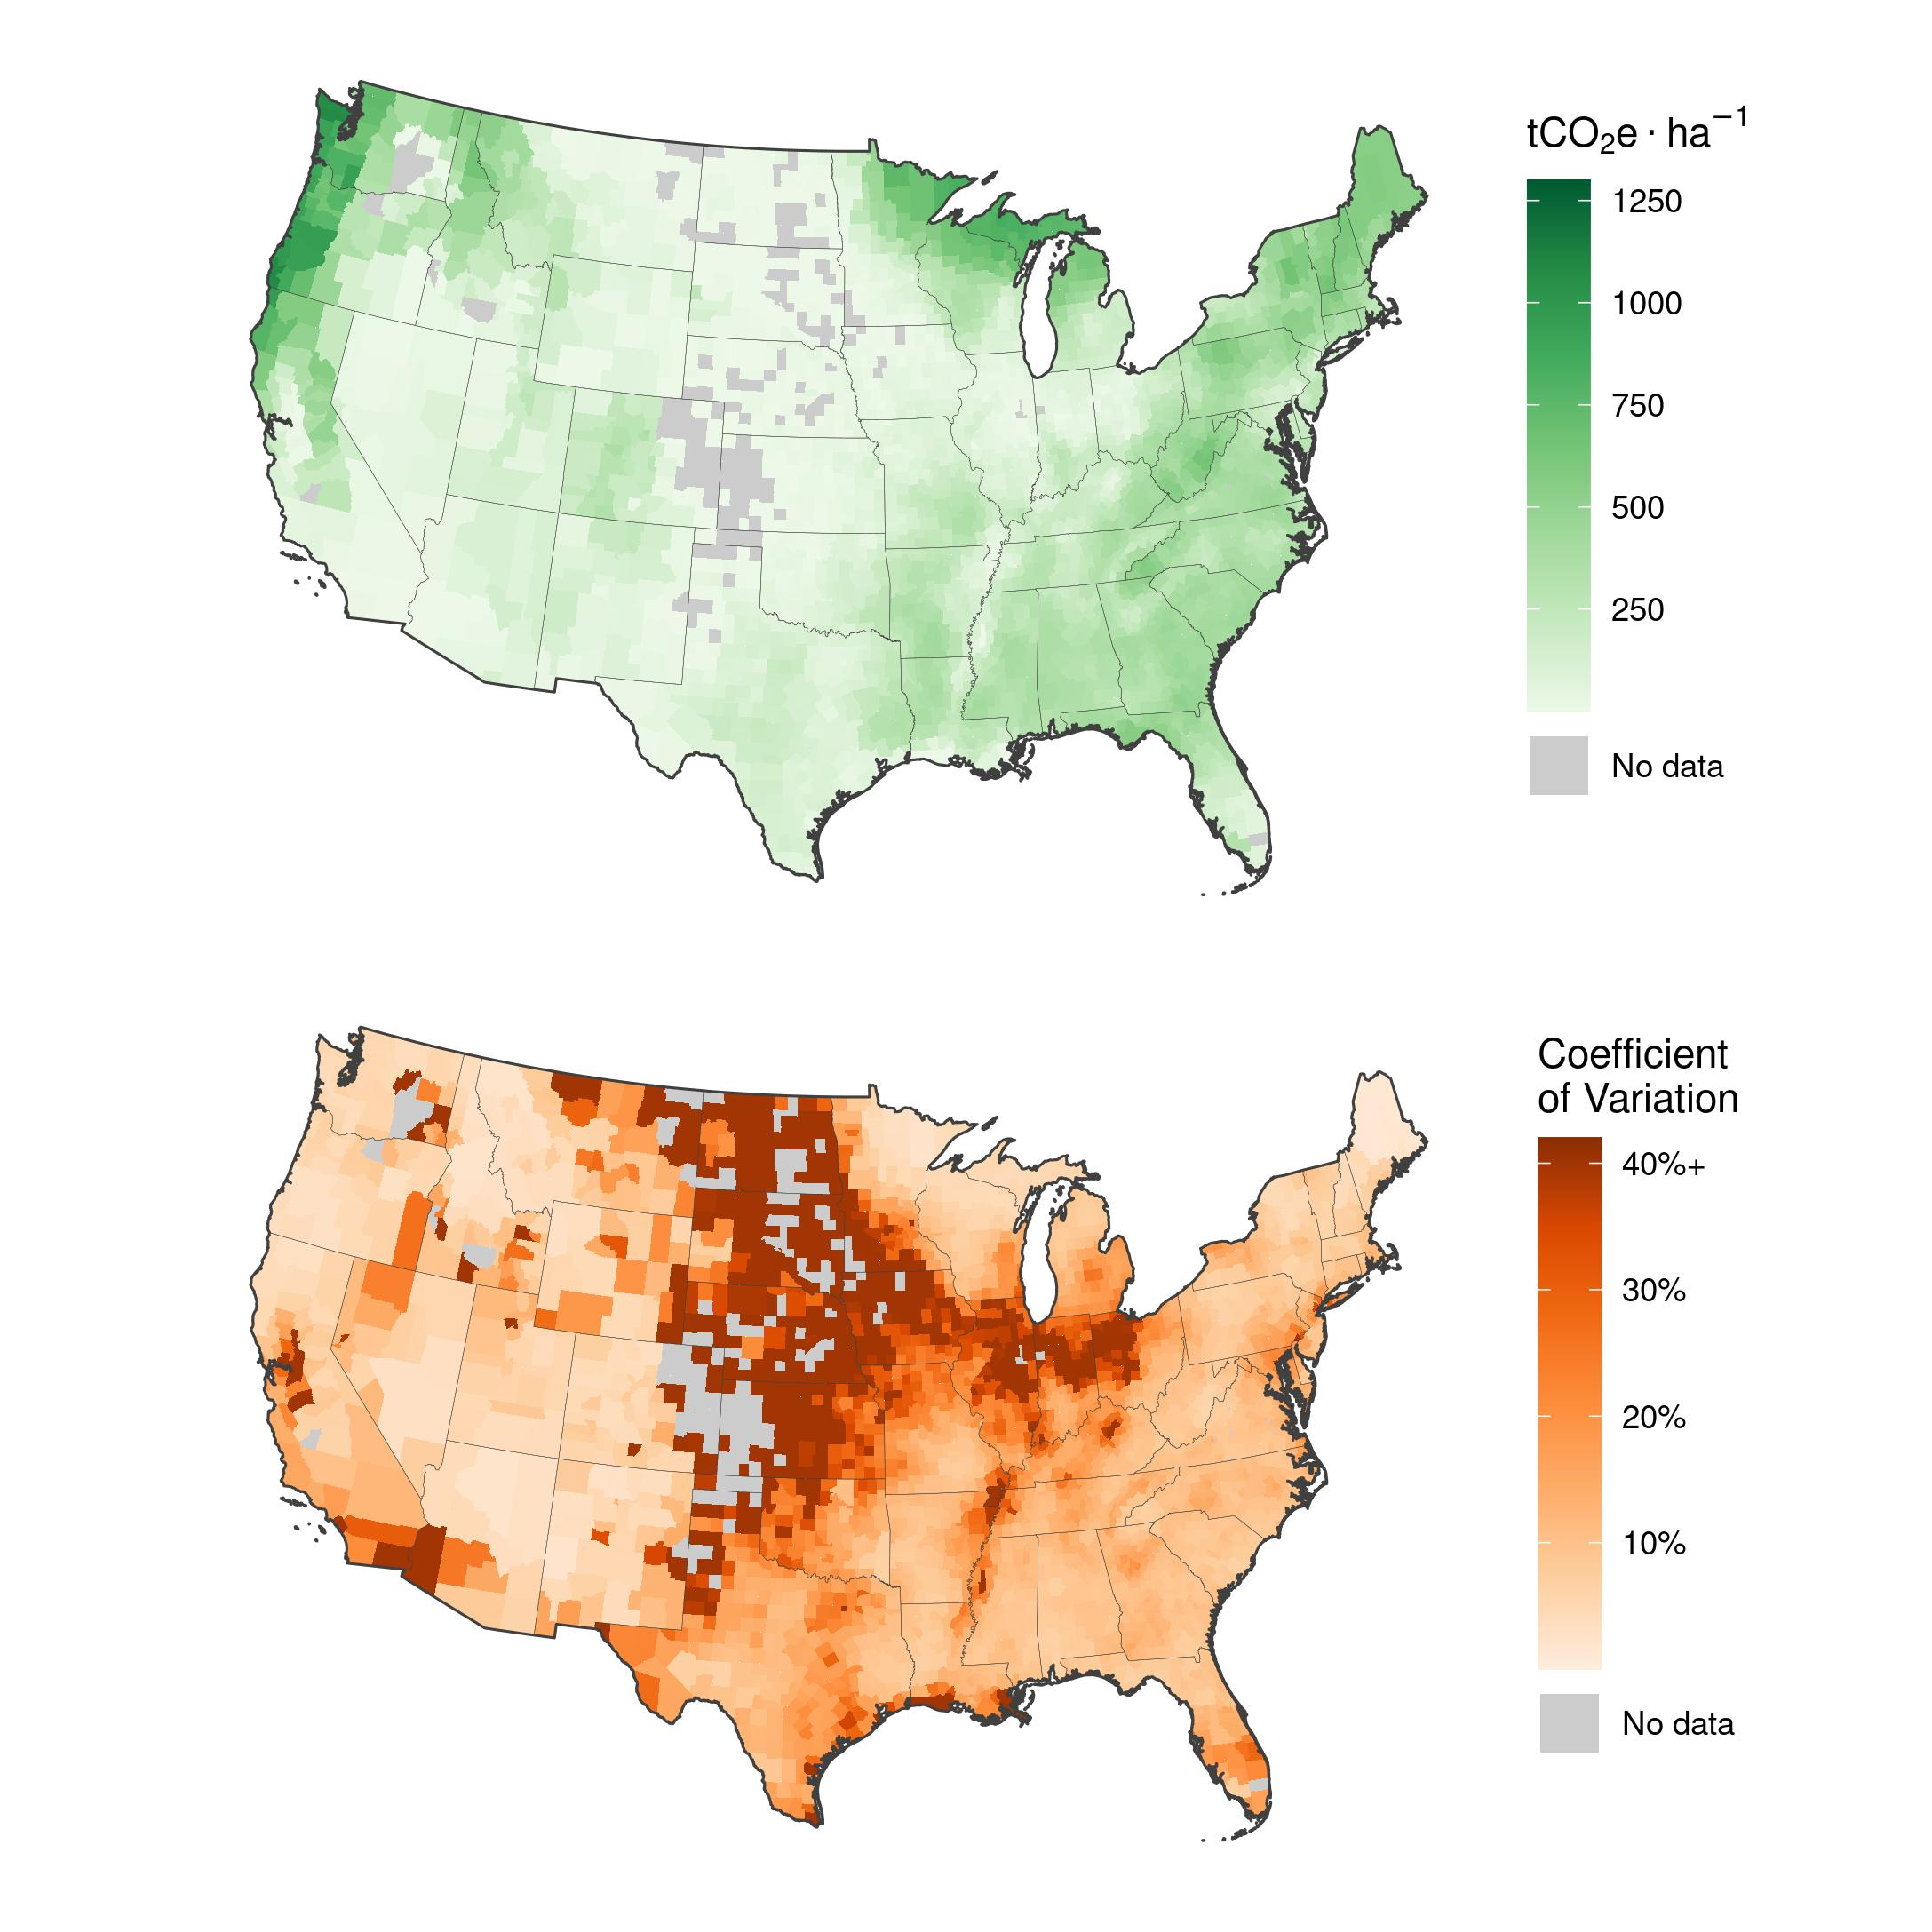
\includegraphics[width=6in]{figure1.jpg}
    \caption{County-level estimates of mean forest carbon density (tons $\mathrm{CO_2}$ equivalent per hectare, $\mathrm{tCO}_2\mathrm{e} \cdot \mathrm{ha}^{-1}$) produced by the spatial Fay-Herriot model with climate predictors (top), and associated coefficient of variation (\%; bottom). Gray shaded counties indicate no forested FIA plots were encountered in the county during the most recent current volume inventory, i.e., direct estimator of total forest carbon and associated variance for the county are equal to zero.}
    \label{fig:smoothed}
\end{figure}

\begin{figure}[t!]
    \centering
    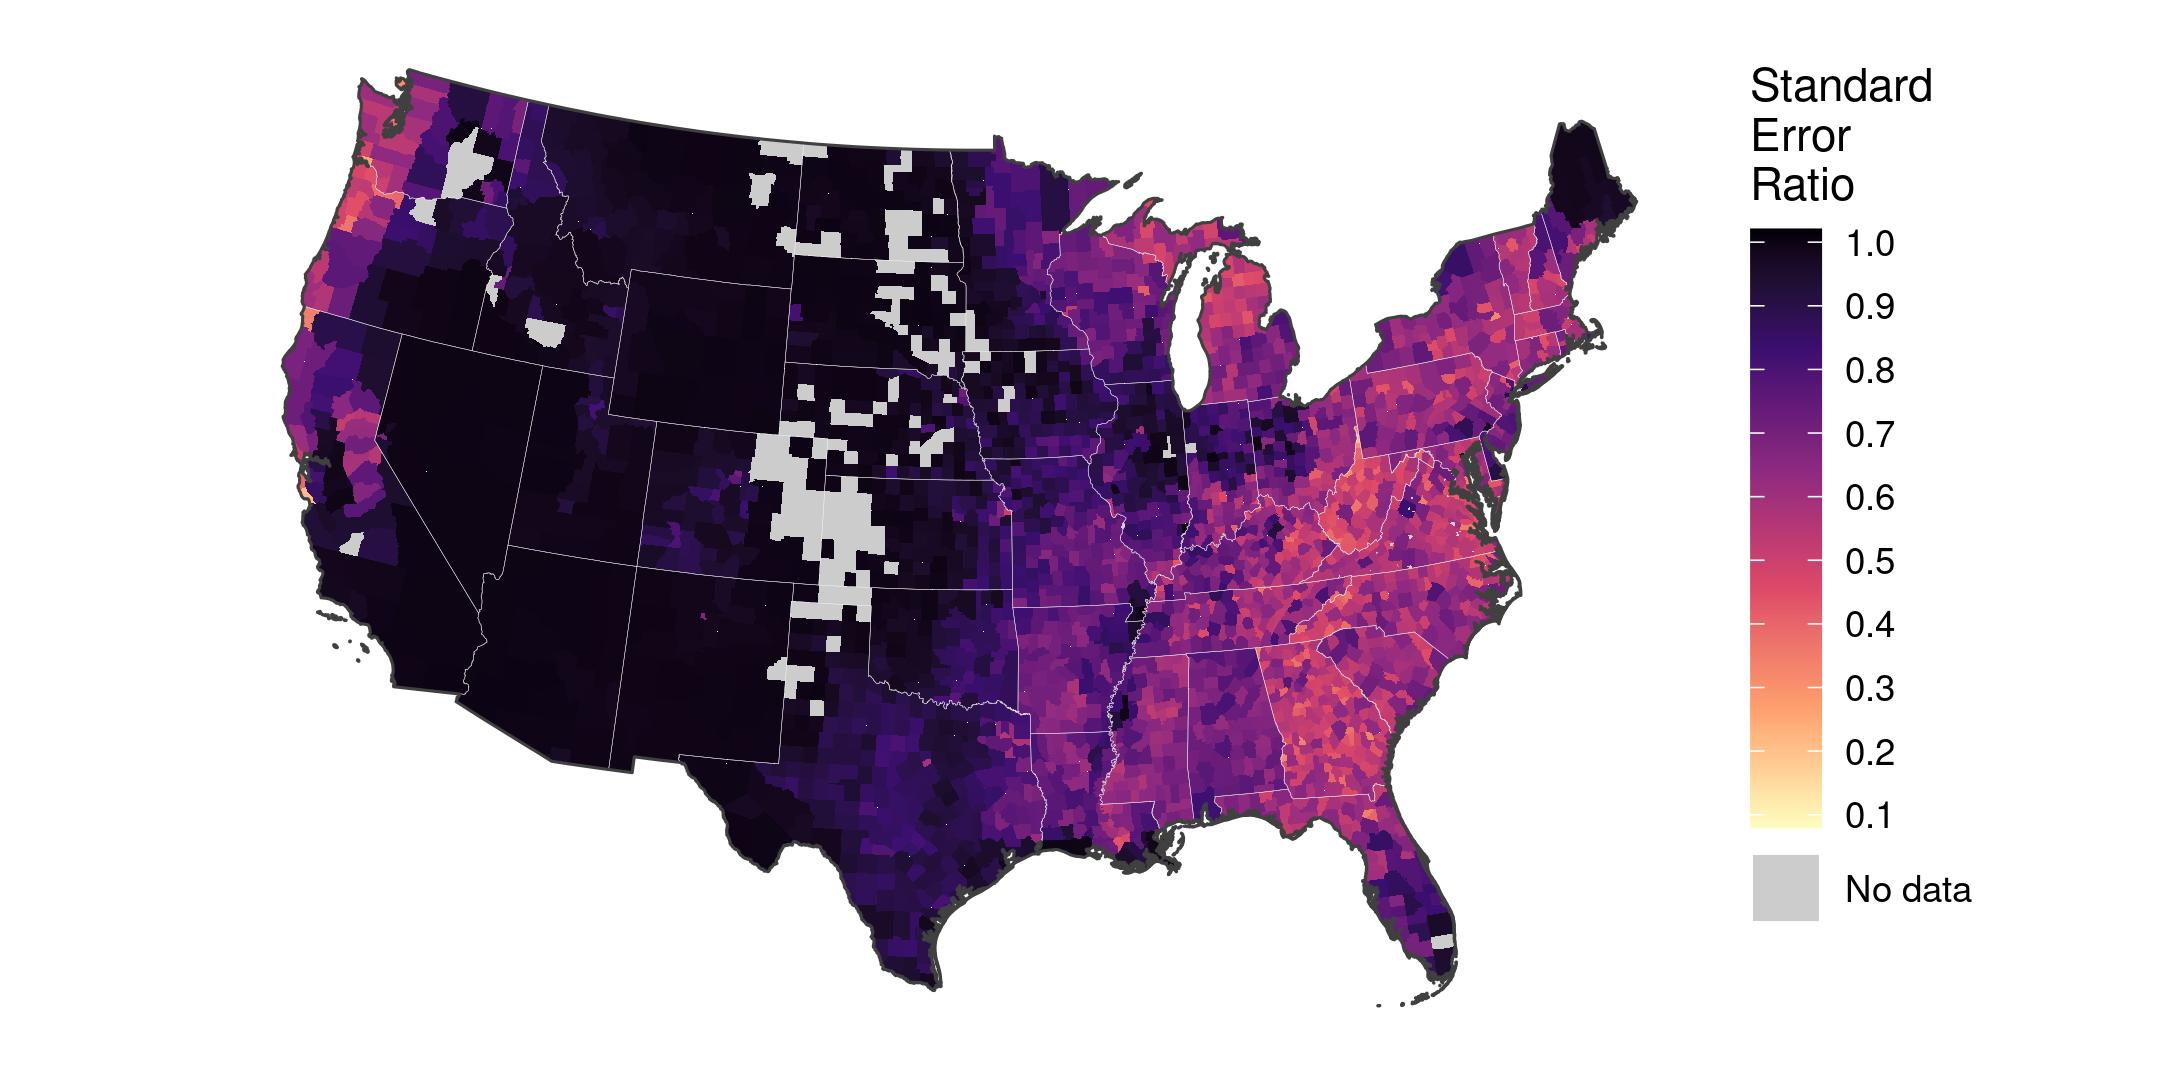
\includegraphics[width=6in]{figure2.jpg}
    \caption{County-level ratios of the standard error of the spatial Fay-Herriot model-based estimator of mean forest carbon density, relative to that of the periodic post-stratified estimator (i.e., FIA's temporally-indifferent estimator). Ratios less than one indicate the model-based approach yields a more precise estimator of forest carbon stocks than the traditional design-based approach. Gray shaded counties indicate no forested FIA plots were encountered in the county during the most recent current volume inventory, i.e., direct estimator of total forest carbon and associated variance for the county are equal to zero.}
    \label{fig:error}
\end{figure}

\begin{figure}[t!]
    \centering
    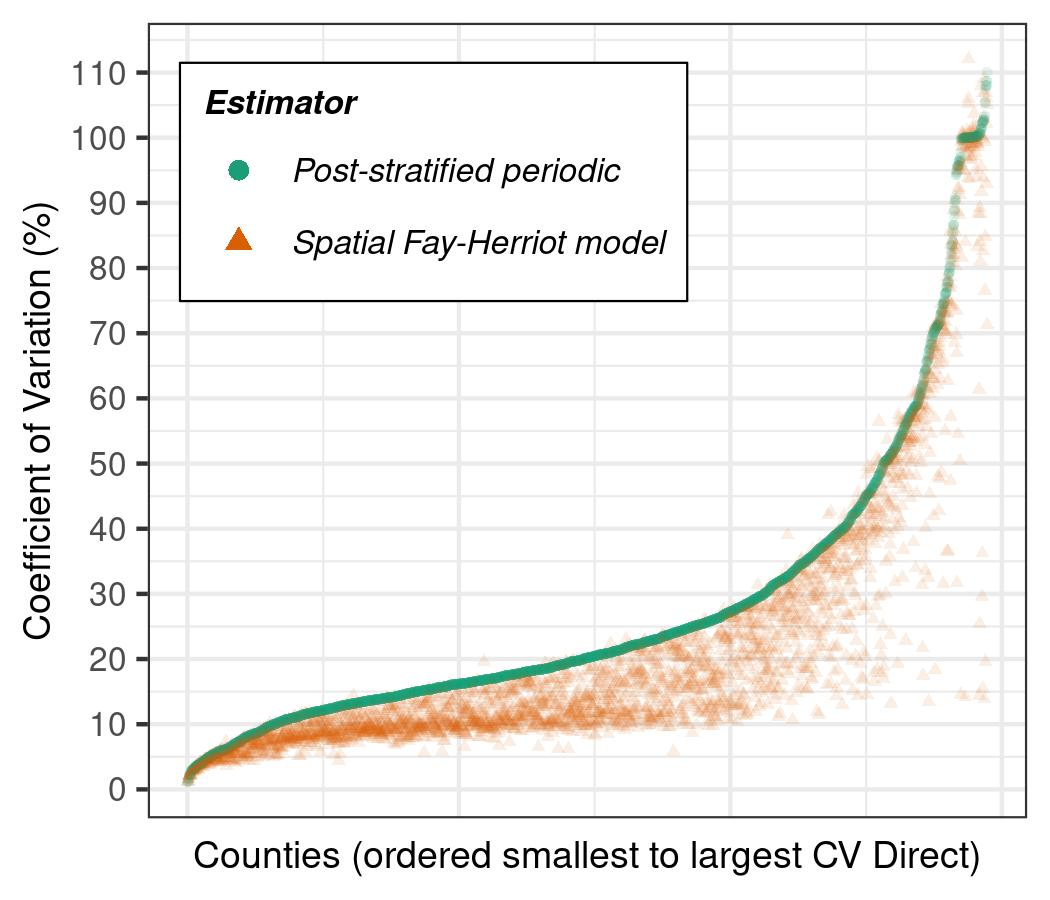
\includegraphics[width=3.5in]{figure3.jpg}
    \caption{Coefficient of variation (\%) of model-based (i.e., spatial Fay-Herriot model) and direct (i.e., post-stratified periodic) estimators of mean forest carbon density by county, ordered by increasing coefficient of variation of the direct estimator.}
    \label{fig:carbon_cv}
\end{figure}

\begin{figure}[t!]
    \centering
    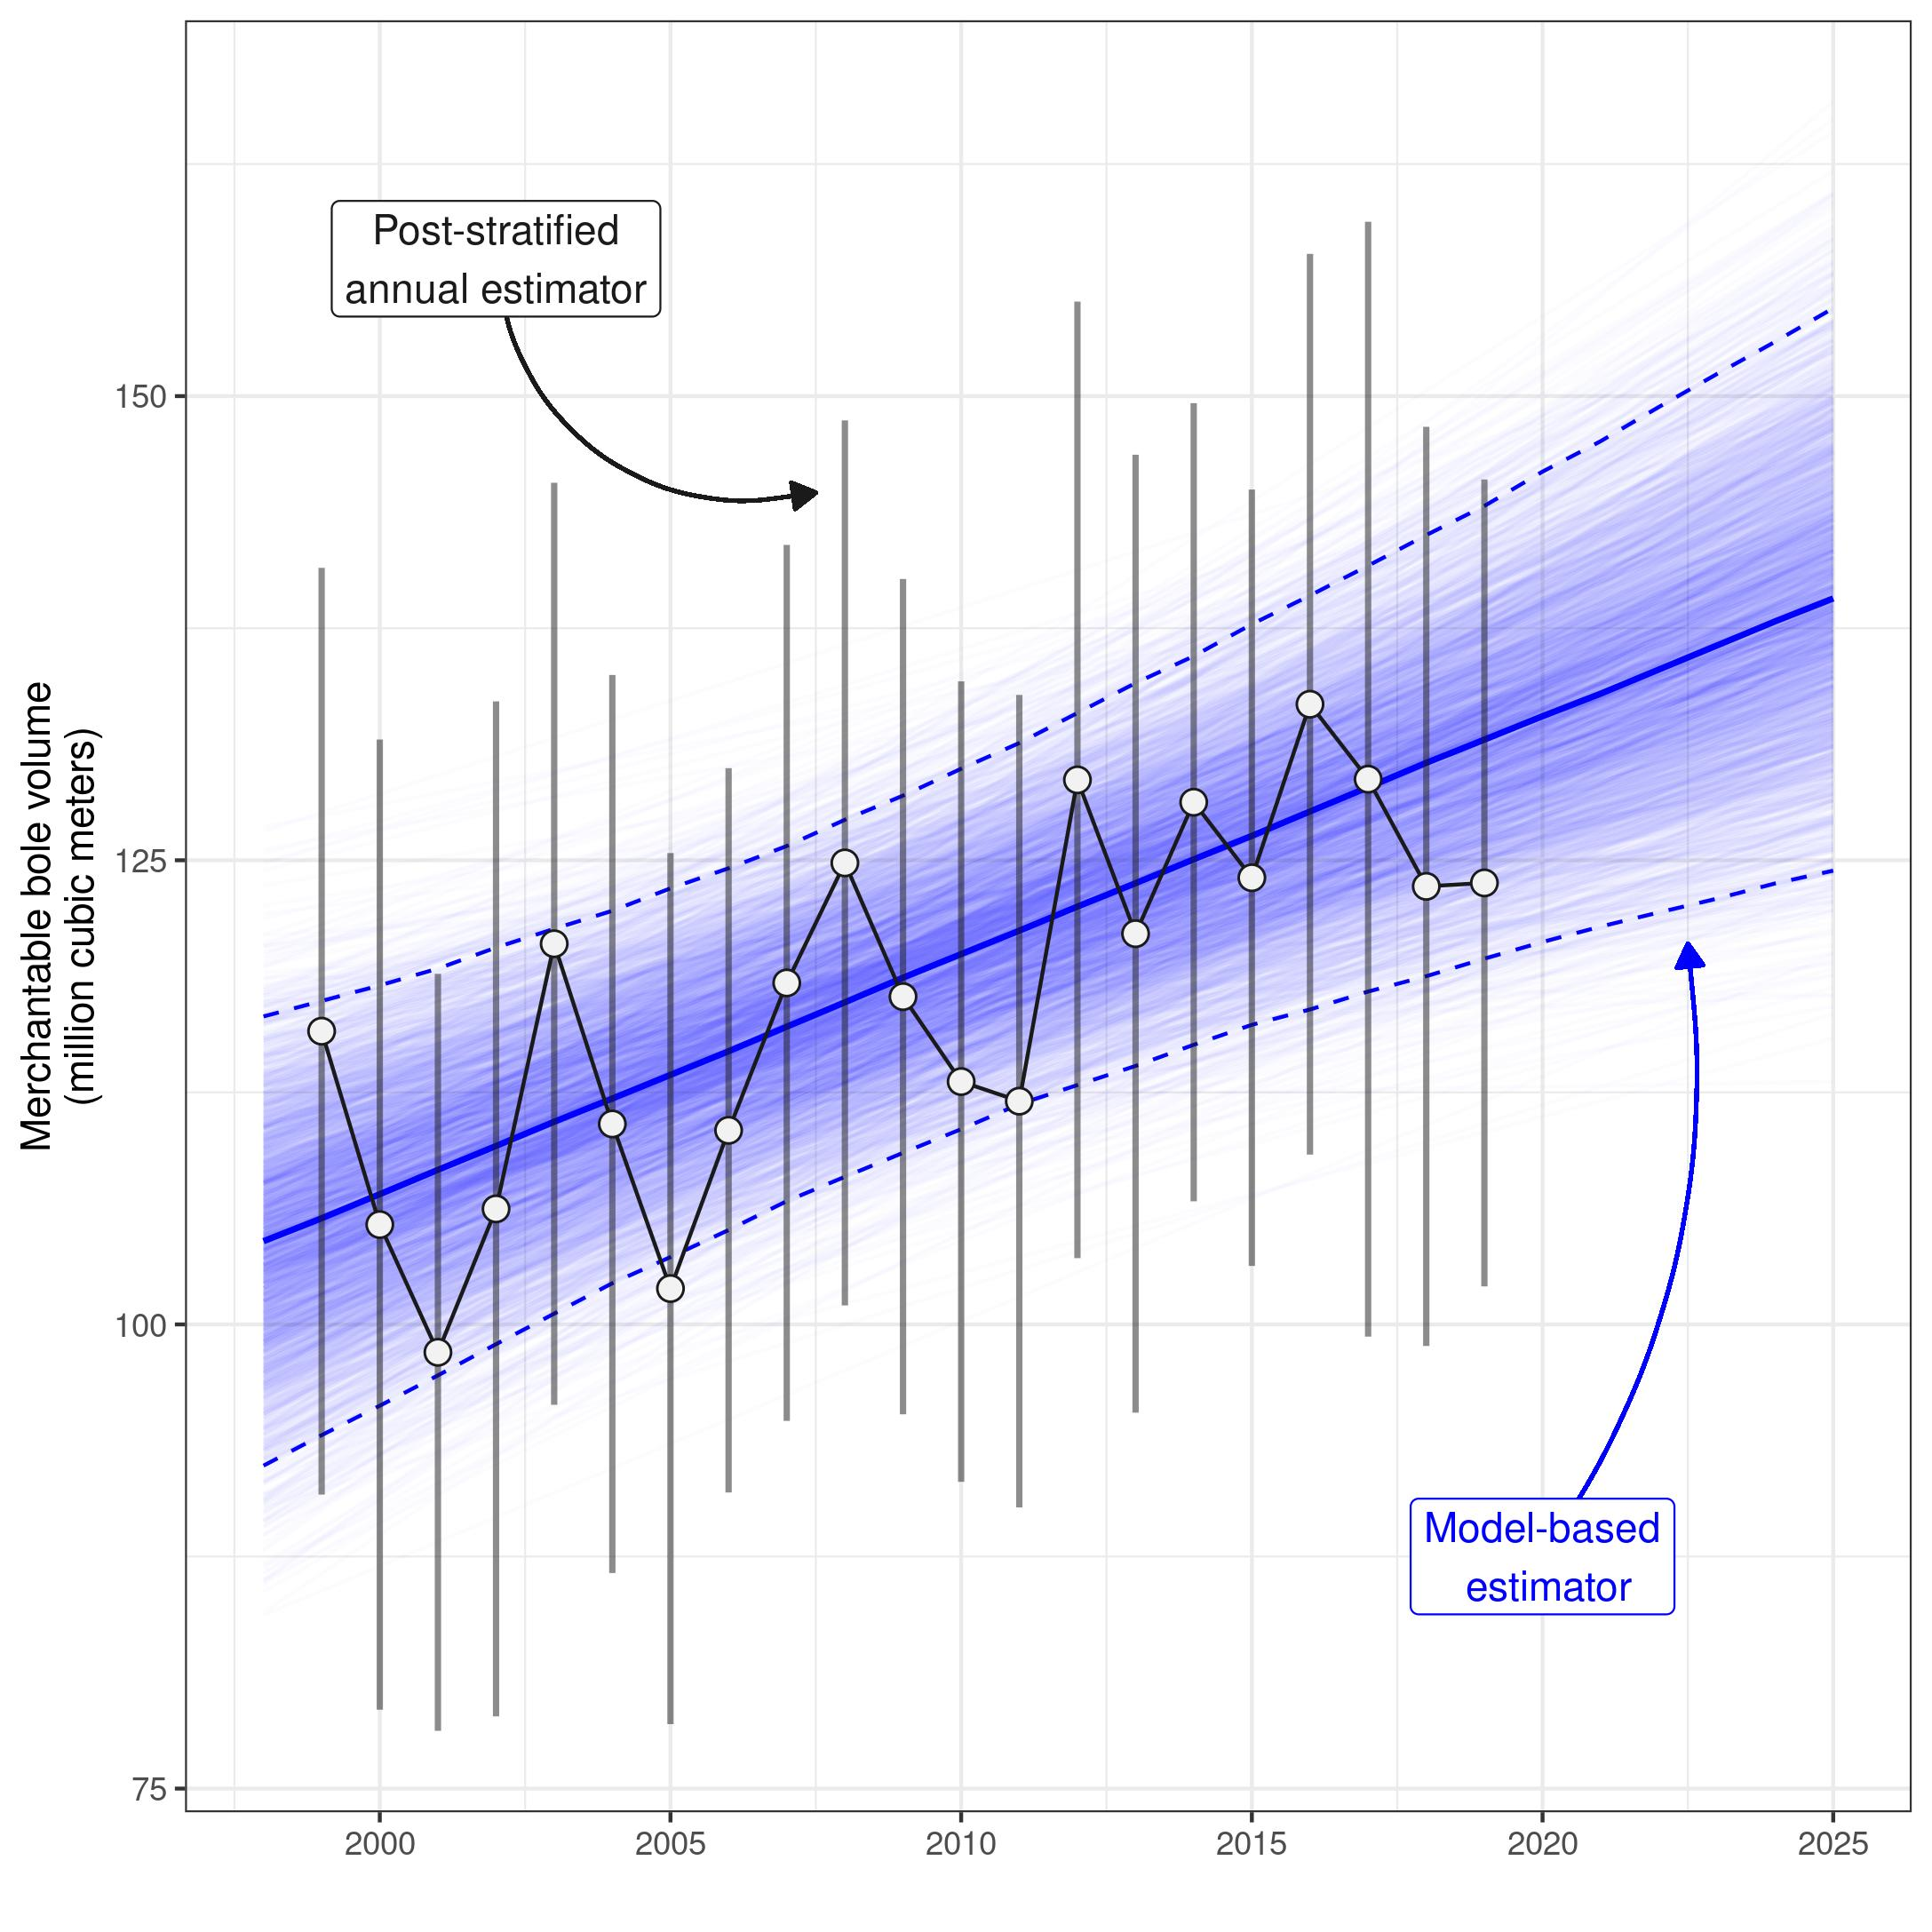
\includegraphics[width=5.5in]{figure4.jpg}
    \caption{Annual model-based and design-based estimates of total merchantable wood volume (million $\mathrm{m}^3$) on timberland in Washington County, Maine. Model-based point estimates are derived from the posterior median of Hamiltonian Monte Carlo (HMC) samples of parameters presented in Eqs \ref{model2:mean}-\ref{model2:total}, and are represented by the solid, dark blue line. Similarly, model-based interval estimates (i.e., Bayesian 95\% credible intervals) are derived from the 2.5\% and 97.5\% quantiles of HMC samples, and are represented by dashed, dark blue lines. Further, realizations of parameters presented in Eqs \ref{model2:mean}-\ref{model2:total} from each HMC sample are represented as thin, semi-transparent blue lines. Hence the posterior predictive distribution of the model-based estimator of total merchantable wood volume can be inferred from the relative density of thin blue lines in a given region of the graph (i.e., higher density of lines indicates higher posterior probability). Annual, design-based point estimates are represented by white circles, and are connected by a solid black line. Design-based interval estimates (95\% confidence intervals) associated with each annual point estimate are presented as vertical gray bars. All design-based estimates were produced using the annual estimator implemented in rFIA \citep{stanke2020rfia}. }
    \label{fig:volume}
\end{figure}

\begin{figure}[t!]
    \centering
    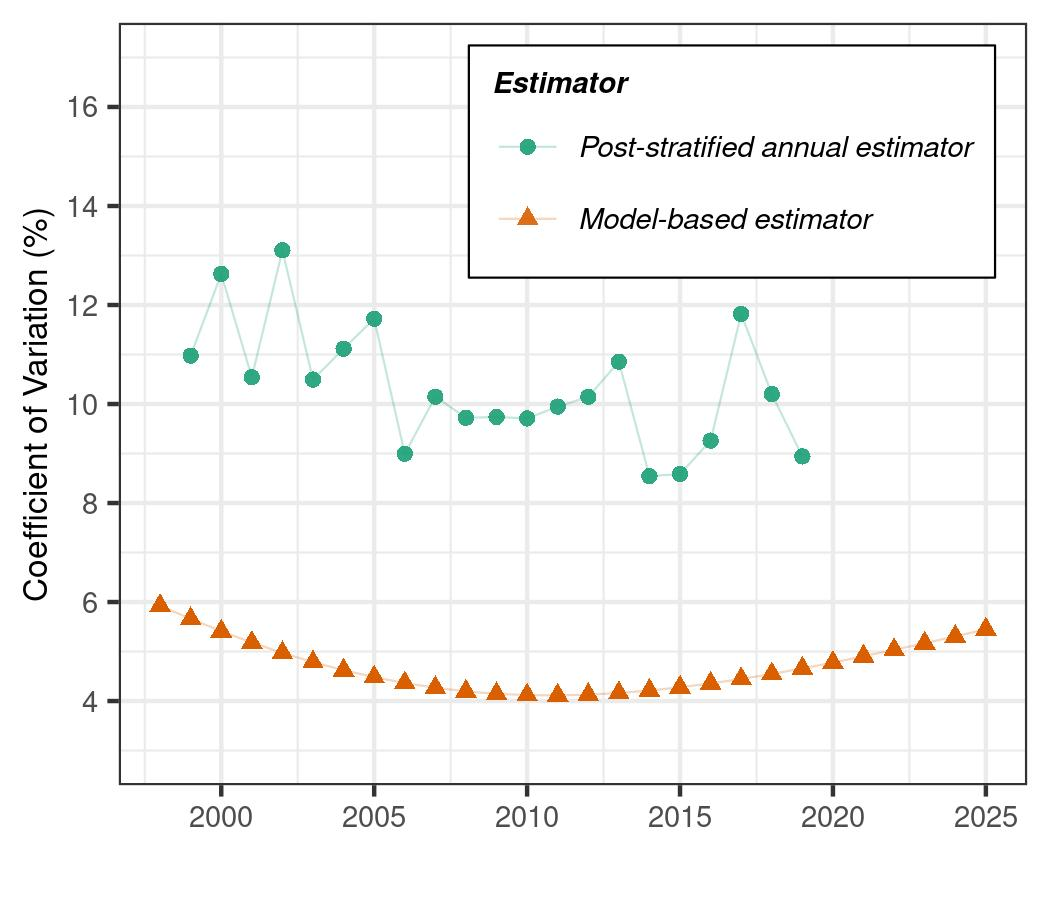
\includegraphics[width=3.5in]{figure5.jpg}
    \caption{Coefficient of variation (\%) of model-based and direct (i.e., post-stratified annual) estimators of trends total merchantable wood volume on timberland in Washington County, Maine.}
    \label{fig:volume_cv}
\end{figure}

\section*{Results}

Results from design-based and model-based estimators are often not strictly comparable due to fundamental differences in their underlying inferential paradigms, see, e.g., \citet{little2004model}. Even among model-based estimators, frequentist and Bayesian inferences yield different interpretation in some cases, see, e.g., \citet{gelmanbda04bda}. Therefore, comparing results derived from these different paradigms, presented in subsequent sections, should be received with an understanding about the respective modes of inference. For example, in some cases we compare design-based direct estimate derived confidence intervals to Bayesian model-based credible intervals. While it can be convincingly argued such comparisons are not appropriate, we present comparative results to explore general patterns in estimates and highlight estimators' qualities.

\subsection*{County-level forest carbon stocks}
Our results indicate the EBLUP derived from the spatial Fay-Herriot model (described in Eqs \ref{model1a}-\ref{model1c}) offers considerable improvements in precision relative to the direct, post-stratified estimator of county-level forest carbon stocks across much of the CONUS. We present model-based estimates of mean forest carbon density, along with associated estimates of precision, in Figure \ref{fig:smoothed}. Similarly, we map the spatial distribution of the SER in Figure \ref{fig:error}. Finally, we illustrate improvements in relative precision offered by the model-based estimator (i.e., measured by the coefficient of variation), along a gradient of relative precision in the direct estimator, in Figure \ref{fig:carbon_cv}.

The spatial Fay-Herriot model yields a spatially smooth estimator of county-level forest carbon stocks, that generally reflects the distribution of forestland across the CONUS (Figure \ref{fig:smoothed}). The largest estimated forest carbon densities are in the coastal Pacific Northwest, Northern Lake States, and Appalachian regions. In contrast, the smallest estimated forest carbon densities appear in the Southwest, Great Basin, and Northern Plains. We show the relative precision of the model-based estimator generally decreases with estimated mean forest carbon density (i.e., lower precision in counties with low carbon density relative to high carbon density) and with county size (i.e., lower precision in small counties relative to large counties) (Figure \ref{fig:smoothed}). Notably, we show the relative precision of the model-based estimator was generally smallest in the Northern Plains and Southern Lake States regions, likely arising from a combination of small county sizes and relatively low forestland area.

We show the model-based estimator of forest carbon stocks offered the greatest improvements in precision in the coastal Pacific Northwest and eastern US, relative to the direct estimator (Figure \ref{fig:error}). In these regions, the SER commonly fell below 0.5, indicating the standard error of the model-based estimator was less than half that of the direct estimator for a given county (i.e., doubling in precision). Across the Interior West, in contrast, we show the model-based estimator rarely improved precision by more than 10\% (i.e., SER commonly exceeded 0.9). Further, results presented in Figure \ref{fig:carbon_cv} indicate the model-based estimator generally offered consistent improvements in relative precision over the direct estimator, regardless of the absolute magnitude of the direct estimator's relative precision.  

\subsection*{Trends in merchantable wood volume in Washington County}
%% Model-based estimator offers improvements in precision, and appears unbiased. Average percent change in the coefficient of variation, we're looking at close to a doubling in precision. 
Our results indicate the model-based estimator of total merchantable wood volume in Washington County, Maine (approach described in Eqs \ref{model2}-\ref{model2:total}) offers substantial improvements in precision relative to the annual, post-stratified estimator (Figures \ref{fig:volume}-\ref{fig:volume_cv}). Specifically, we show 95\% credible intervals associated with model-based point estimates are consistently narrower than 95\% confidence intervals associated with the direct estimator (Figure \ref{fig:volume}). On average over the period 1999-2019, the coefficient of variation of the model-based estimator was 55.9\% lower than that of the direct estimator (ranging from 48.9\%-62.4\% lower across all years) (Figure \ref{fig:volume_cv}), indicating the model-based estimator is more than twice as precise as the direct estimator for our population of interest. Further, consistent alignment of direct and model-based point estimates suggests the model-based estimator is generally unbiased for the domain of interest (Figure \ref{fig:volume}). 

%% Trends, interpretation of parameter estimates
Both approaches indicate that total merchantable wood volume in Washington County has increased considerably over the period 1999-2019 (Figure \ref{fig:volume}). Notably however, the model-based approach yields a smooth, linear estimator of trends in total merchantable volume. The direct estimator, in contrast, exhibits unrealistic rates inter-annual variability ($\pm$5-10\% per year, arising from sampling) and pronounced cyclical patterns over the same period (arising from remeasurement of annual panels). Further, the model-based estimator offers an intuitive approach to characterizing the magnitude, direction, and statistical significance of temporal trends in our variable of interest---a feature the direct estimator lacks (absent estimating change from remeasured panels). Specifically, the posterior distribution of the adjusted population-level regression coefficient, $\hat{\beta}$, yields an estimator of average annual change in total merchantable wood volume across our domain of interest. The posterior median of $\hat{\beta}$ was 1,293,900$\mathrm{m}^3 \cdot \mathrm{yr}^{-1}$ (95\% credible interval: 588,000-1,989,000$\mathrm{m}^3 \cdot \mathrm{yr}^{-1}$), indicating a relatively rapid increase total merchantable wood volume over the last two decades. Further, we show the probability that $\hat{\beta}$ exceeds 0 is $>0.999$, indicating very high certainty in the observed upward trend.  

%% Ability to predict to unobserved domains, with measurable uncertainty. 
Finally, the model-based approach offers the ability to forecast future changes in our variable of interest, along with measurable estimates of uncertainty. We highlight this unique capacity in Figures \ref{fig:volume} and \ref{fig:volume_cv} by predicting total merchantable wood volume, along with estimates of relative precision, over the period 2020-2025---years for which no FIA data has yet been collected/released for our domain of interest. By the year 2025, we estimate, with 95\% probability, that total merchantable wood volume on timberland in Washington County, Maine will range between 124.4-154.7$\mathrm{m}^3$, conditional on proper specification of our model. 



\section*{Discussion}
%% FIA has experienced considerable increases in demand for small area estimates, and a shift from traditional estimation paradigms will be required to meet demand. %% rFIA can help accelerate this transition
The FIA program operates the largest network of permanent forest inventory plots in the world, making it well suited to provide critical information on US forests over large geographic and temporal domains (e.g., periodic, state-level estimates). However, the program has experienced increased demand for estimates of forest variables for smaller spatial and temporal domains than traditional sample-based estimation approaches can deliver. Providing such estimates without additional investments in field sampling requires adopting alternative estimation approaches. Here, we presented two case studies that demonstrated some aspects of rFIA's potential to simplify application of SAE to data collected by the FIA program, and thus accelerate adoption of such techniques by FIA data users.

%% Brief discussion of area-level model. Who else has used these models? Focus on the potential extensions - could easily be spun into a spatio-temporal model using annual county-level estimates
First, we estimate contemporary county-level forest carbon stocks across the CONUS using an area-level spatial Fay-Herriot model (Figure \ref{fig:smoothed}), and show the model-based approach offers considerable gains in precision across the predominately forested regions of the CONUS (Figure \ref{fig:error}). Previous efforts have applied spatial Fay-Herriot models to FIA data to improve precision of estimators of forest density variables \citep{goerndt2011comparison}, private landowner characteristics \citep{ver2017hierarchical}, and forestland removals \citep{coulston2021enhancing}. Area-level models are particularly useful when inventory plot locations are unknown or measured imperfectly, as spatial auxiliary data need not be associated with plot locations, but rather with the areal units \citep{rao2015small, mauro2017analysis}. That is, spatial predictors can be used in area-level models without requiring the release of actual FIA plot locations. We provide all code and data used to develop the area-level model presented herein on GitHub (\url{https://github.com/hunter-stanke/FGC_rFIA_SAE}) and at our official website (\url{https://rfia.netlify.app}). Our procedures can be easily adapted for use with alternative state variables, spatial domains, and/or auxiliary data, and we encourage interested users to adapt our code for use in their own applications of area-level SAE models.

%% Brief discussion of unit-level model. Again, focus on the extensions. We're limited in terms of incorporating spatial predictors here, as neither the plot locations or stratum boundaries have been released.
Second, we follow the approach presented in \citet{little2004model} to develop a temporally-explicit unit-level estimator of multi-decadal trends in merchantable wood volume in Washington County, Maine, using a Bayesian mixed-effects model. We show the model-based approach offered substantial improvements in precision of annual estimates, relative to the traditional, post-stratified approach (Figures \ref{fig:volume}-\ref{fig:volume_cv}). Further, we show the model-based estimator offers an intuitive approach to characterizing the magnitude, direction, and statistical significance of temporal trends, and allows predictions of the state variable to be made to unobserved domains, with measurable uncertainty (e.g., forecast future change). Unit-level SAE models have been widely applied to FIA data in recent decades \citep{goerndt2011comparison, mcroberts2017multivariate, ohmann2002predictive, babcock2018geostatistical}, and frequently draw from remotely-sensed auxiliary variables to support domain estimation. However, extending the approach presented herein to incorporate spatial auxiliary data will present challenges for most users of FIA data, as neither the true locations of inventory plots, nor the spatial boundaries of strata used for post-stratification are available in the public version of the FIA Database. Nevertheless, the unit-level model presented can be easily adapted for applications involving alternative populations of interest, and might be useful in the detection and characterization of long-term change in forest ecosystems. Further, such models can be used to characterize the status and change in forest variables at spatial and/or temporal domains that are not currently possible using sample-based approaches (e.g., stand-level estimates). Once again, we provide all code and data used to develop the unit-level model presented herein on GitHub (\url{https://github.com/hunter-stanke/FGC_rFIA_SAE}) and at our official website (\url{https://rfia.netlify.app}). 

\subsection*{Role of rFIA in accelerating the adoption of SAE techniques for FIA data}
%% We make things easier in three primary ways
%% Spatial area-level models with TI
%% Temporal and/or spatial-temporal area-level models with ANNUAL
%% Plot-level summaries and design info for unit-level models
We posit that rFIA has the potential to simplify application of model-based SAE techniques to FIA data in three key ways. First, rFIA implements standard, periodic post-stratified estimators---consistent with the estimators implemented by FIA's popular online estimation tool, EVALIDator \citep{evalidator}---within highly flexible, user-defined domains. These direct estimators, along with their associated variances, form the basis for construction of area-level estimators, as demonstrated by our spatial Fay-Herriot model \citep{fay1979estimates, petrucci2006small, pratesi2008small} of county-level forest carbon stocks. Second, rFIA implements annual post-stratified estimators, offering increased temporal specificity over standard periodic estimators (i.e., the temporally-indifferent estimator), and supporting the development of small area estimators that require direct annual estimates of forest variables at aggregate scales. Examples of such temporally-explicit, area-level estimators include mixed-estimators \citep{van1999modeling} and the spatial-temporal Fay-Herriot model \citep{marhuenda2013small}. Finally, rFIA allows summaries of forest variables to be returned for individual response units (i.e., plot-level) and provides utility functions for extracting design information relevant to particular inventory cycles (e.g., stratum assignments and weights). Together, these data can be used to construct a wide variety of unit-level estimators that acknowledge features of FIA's survey design, as demonstrated in our mixed-effects model of trends in merchantable wood volume in Washington County, Maine. 

%% Our goal is to provide the data, and let the user take advantage of existing tools for small area estimation. 
Adoption of SAE methods by FIA data users (particularly new users) is limited more by FIA's complex data structure and inventory design than by the availability of tools that implement SAE methods. Thus, we argue the primary benefit of rFIA in accelerating SAE method adoption is its ability to simplify the process of summarizing and formatting FIA data to serve as input to a wide variety of SAE models. There is a large suite of existing, open-source tools that provide generalized implementations of many area-level and unit-level SAE models. For example, the sae R package \citep{molina2015sae} is specifically designed to implement area-level SAE models, and we draw from this functionality to develop the area-level model of forest carbon stocks presented herein. Our intention is not to duplicate efforts of others by implementing common SAE models natively in rFIA, but rather to reduce barriers to the application of such SAE models to FIA data that arise from the complexity of FIA's data structure and sampling design. 

\subsection*{Future extensions of rFIA}
%% The immediate focus is on time, as it's easier to provide canned estimators for temporally-specific approaches
Current efforts to extend rFIA include the implementation of a suite of model-based time-series estimators that aim to improve the precision of annual estimates of forest variables, thereby increasing the relevance of FIA data for change detection, characterization, and attribution. Specifically, we aim to provide an intuitive implementation of Van Deusen's mixed-estimator \citep{van1999modeling}, which was recently shown by \citet{hou2021updating} to offer considerable improvements in the precision of annual FIA-based forest land area estimates, at both the state- and county-levels. Further, we aim to provide an alternative Bayesian estimator of annual trends in forest variables based on a measurement error model (e.g., similar to Bayesian meta-analysis \citep{sutton2001bayesian}). Notably, both approaches effectively smooth annual, post-stratified estimates of forest variables, and hence are compatible with FIA's existing inventory design and database structure. 



\clearpage

\printbibliography

\end{document}

